\documentclass{article} 
\usepackage{tikz-qtree}
\usepackage{geometry}
\geometry{verbose,tmargin=3cm,bmargin=3cm,lmargin=1.5cm,rmargin=3cm,headheight=3cm,headsep=3cm,footskip=1cm}
\begin{document}


\begin{tikzpicture}[scale=0.7,every tree node/.style={draw,circle},
   level distance=1.25cm,sibling distance=6.cm, 
   edge from parent path={(\tikzparentnode) -- (\tikzchildnode)}]
\Tree [
    [.1 ]
	[.2 ]
    [.3 ]
    [.4 ]       
    ]
\begin{scope}[xshift=6in,every tree node/.style={},edge from parent path={}]
\Tree [.{} [.{1. trekning} ]]
\end{scope}
\end{tikzpicture}

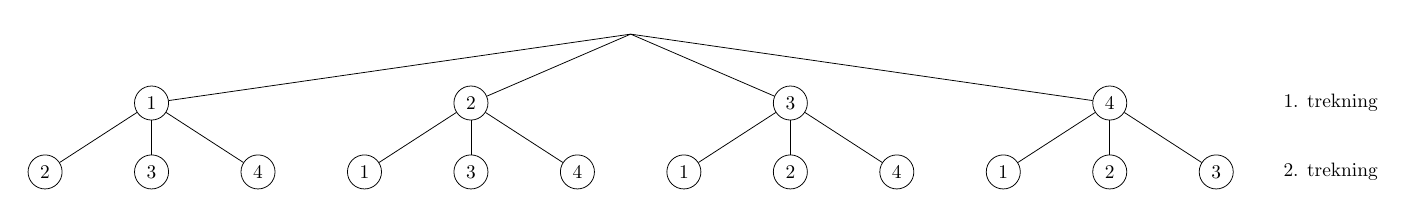
\begin{tikzpicture}[scale=0.7,every tree node/.style={draw,circle},
   level distance=1.25cm,sibling distance=1.3cm, 
   edge from parent path={(\tikzparentnode) -- (\tikzchildnode)}]
\Tree [
    [.1 [.2 ] [.3 ] [.4 ]]
	[.2 [.1 ] [.3 ] [.4 ]]
    [.3 [.1 ] [.2 ] [.4 ]]
    [.4 [.1 ] [.2 ] [.3 ]]       
    ]
\begin{scope}[xshift=5in,every tree node/.style={},edge from parent path={}]
\Tree [.{} [.{1. trekning} [.{2. trekning} ] ]]
\end{scope}
\end{tikzpicture}

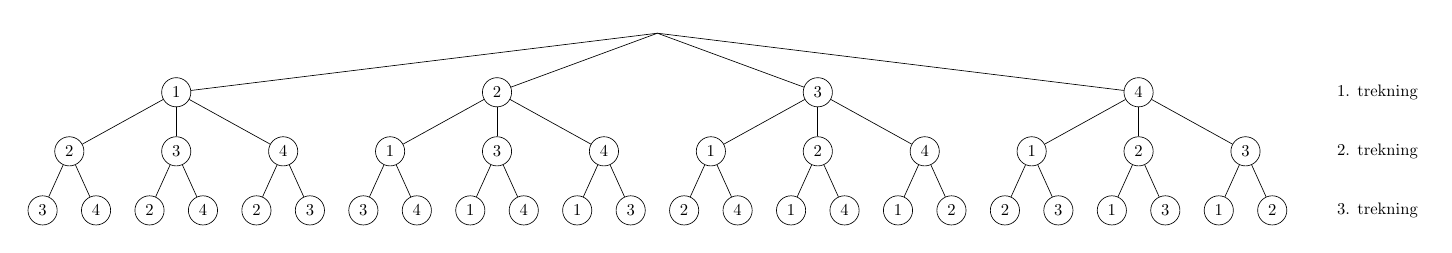
\begin{tikzpicture}[scale=0.6,every tree node/.style={draw,circle},
   level distance=1.25cm,sibling distance=.5cm, 
   edge from parent path={(\tikzparentnode) -- (\tikzchildnode)}]

\Tree [ 
    [.1  
      [.2 [.3 ] [.4 ]] [.3 [.2 ] [.4 ]] [.4 [.2 ] [.3 ]]
    ]
	[.2  
	      [.1 [.3 ] [.4 ]] [.3 [.1 ] [.4 ]] [.4 [.1 ] [.3 ]]
	]
    [.3  
          [.1 [.2 ] [.4 ]] [.2 [.1 ] [.4 ]] [.4 [.1 ] [.2 ]]
    ]
    [.4  
          [.1 [.2 ] [.3 ]] [.2 [.1 ] [.3 ]] [.3 [.1 ] [.2 ]]
    ]       
    ]
\begin{scope}[xshift=6in,every tree node/.style={},edge from parent path={}]
\Tree [.{} [.{1. trekning} [.{2. trekning} [.{3. trekning} ]]]]
\end{scope}
\end{tikzpicture}

\newpage

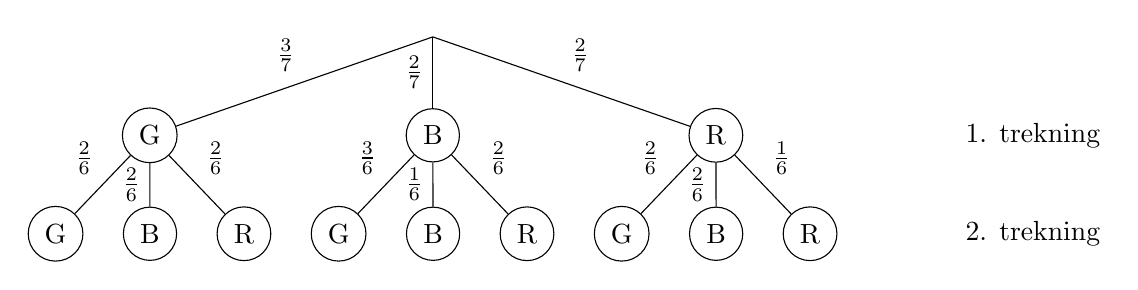
\begin{tikzpicture}[every tree node/.style={draw,circle},
   level distance=1.25cm,sibling distance=.5cm, 
   edge from parent path={(\tikzparentnode) -- (\tikzchildnode)}]
\Tree [ 
	\edge node[auto=right]{$\frac{3}{7}$}; 
    [.G  
      \edge node[auto=right]{$\frac{2}{6}$}; [.G  ]
       \edge node[auto=right]{$\frac{2}{6}$};  [.B ] 
	    \edge node[auto=left]{$\frac{2}{6}$};[.R ]
    ]
    \edge node[auto=right]{$\frac{2}{7}$}; 
    [.B
      \edge node[auto=right]{$\frac{3}{6}$}; [.G  ]
       \edge node[auto=right]{$\frac{1}{6}$};  [.B ] 
	    \edge node[auto=left]{$\frac{2}{6}$};[.R ]
    ] 
    \edge node[auto=left]{$\frac{2}{7}$};
    [.R
      \edge node[auto=right]{$\frac{2}{6}$}; [.G  ]
       \edge node[auto=right]{$\frac{2}{6}$};  [.B ] 
	    \edge node[auto=left]{$\frac{1}{6}$};[.R ]
    ]    
    ]
\begin{scope}[xshift=3in,every tree node/.style={},edge from parent path={}]
\Tree [.{} [.{1. trekning} [.{2. trekning} ]]]
\end{scope}
\end{tikzpicture}
\end{document}